\documentclass[journal]{IEEEtran}

\usepackage{graphicx}
\usepackage[utf8]{inputenc}




\begin{document}

\title{\textbf{loss weighting for learnability imbalance in multiclass-classification}}



\author{Theodor Peifer
        \linebreak
        email: thp7219@thi.de
        \linebreak
        Technische Hochschule Ingolstadt
}



\maketitle


\begin{abstract}
Neural Networks have proven themselves to be powerful classification 
tools by solving problems in a range of domains with high accuracy. 
But especially when it comes to multi-class classification the accuracy is never evenly distributed across all classes, which means that the true-positive rate for each class separately is different.
This can happen even in balanced datasets since some classes are more difficult to learn by the model than others (this phenomenon is further referred to as \emph{learnability-imbalance}).
A common way to address this problem is to give a weight to the error function for each class to penalize losses of certain classes higher or lower.
This research will address the determination of such weights to counteract the learnability-imbalance of class-balanced data sets using previously calculated evaluation scores of the same model.
Therefore the goal is to find methods to lower the variance of the true positive rates of each class.
\end{abstract}


\section{Introduction}
When working with unbalanced datasets it is common to weight the loss functions [1] based on the percentage of elements per class that make in the whole dataset in order to prevent that one class is learned 
excessively worse than others.
For each class, the error function will multiply the loss of its samples with the correspoding weight which leads to the enlargement of the error. 
Since the aim of a neural network is to minimize that error, samples that produce a high loss will receive a higher focus.
But this learnability imbalance appears also on balanced dataset for a vareity of reasons, for example when the quality of the data of a class is lower than the rest of the data. 
A second reason, that will be presented later on, is that when the similiarity of the samples of two classes is high, 
the model can confuse them with each other what will often result in a lower accuracy of both classes.
The question is how to create loss weights for a model that gets trained on a balanced data set. To determine the learnability differences of the individual classes, the model must first be trained and evaluated normally and unweighted.
The evaluation will produce a set of true positive rates for each class which reveal what classes the model has problems with and should have received a higher weight. 
The figure (1) below shows the true positive rates of a an evaluated image classification model that was trained on the CIFAR-10 dataset, which contains 32 x 32 pixel images of ten different classes [2].
This dataset is a good show case for the learnability imbalance problem since it has similiar classes, such as \emph{dog} and \emph{cat} and will be used as one of the main datasets to run the research experiments on.

\begin{figure}[h!]
        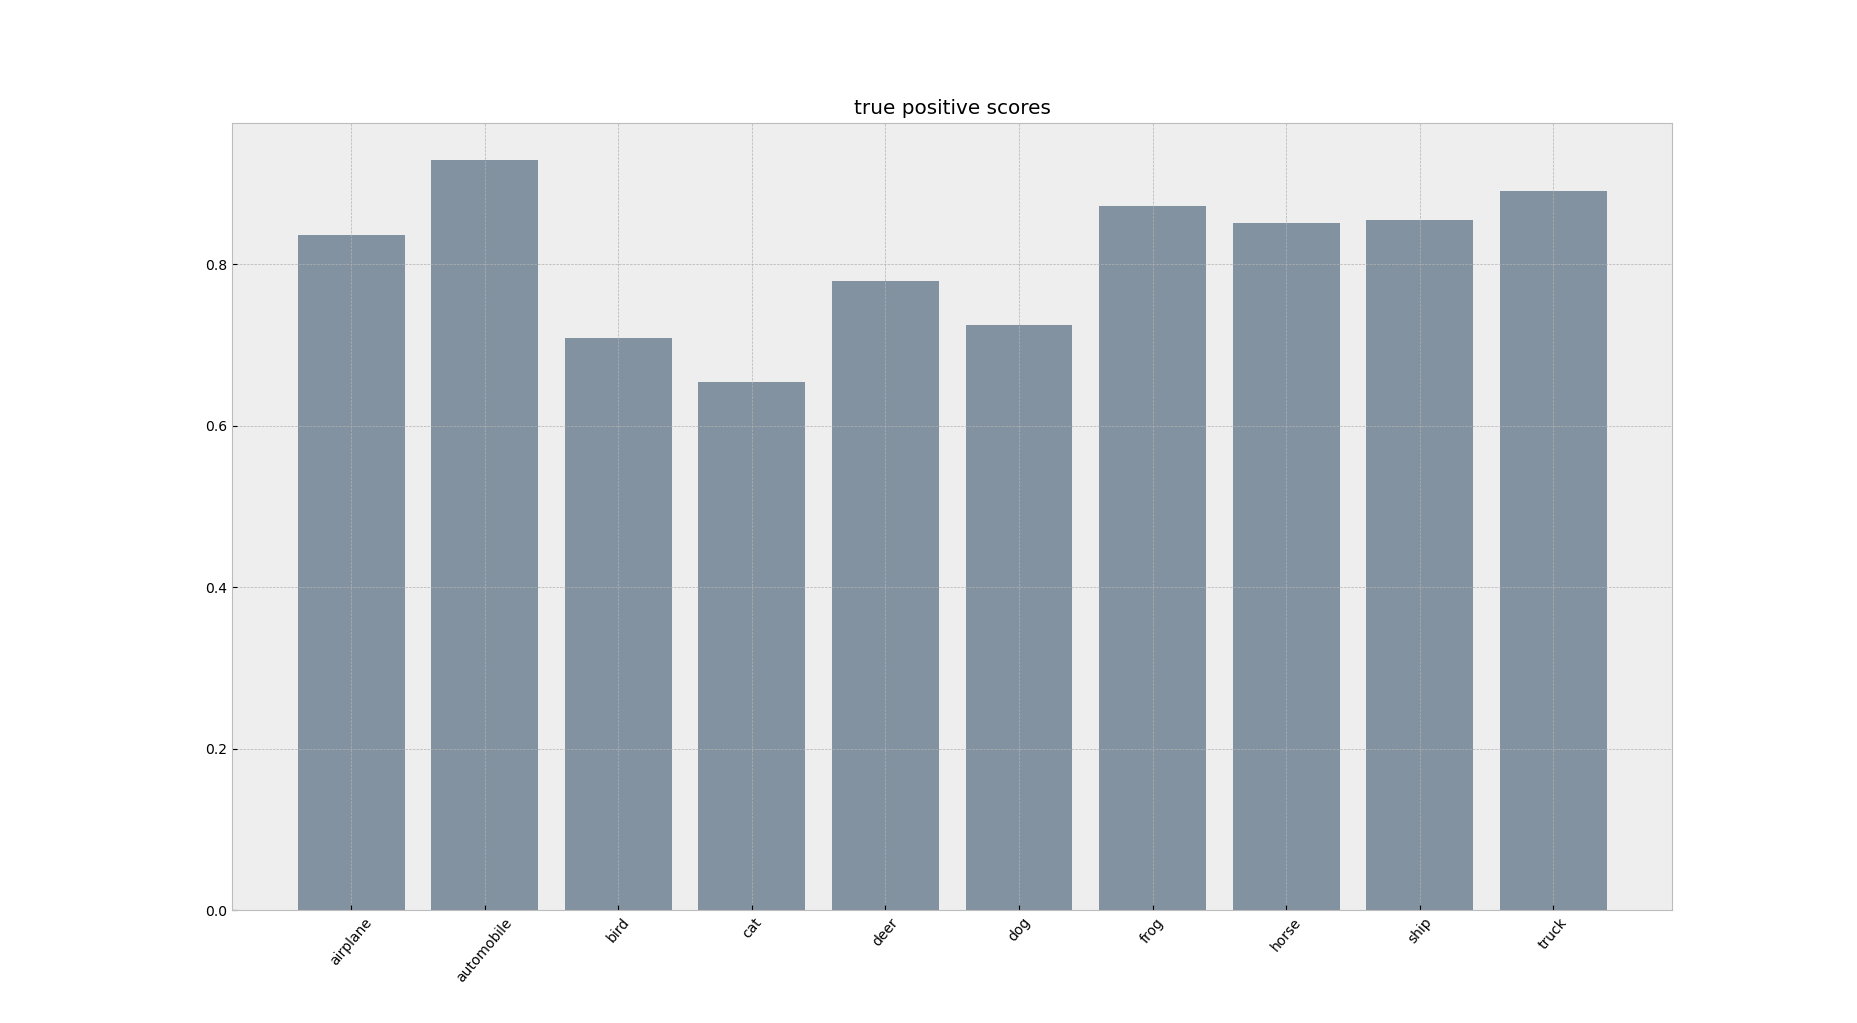
\includegraphics[width=\linewidth]{images/cifar10_tp_scores.png}
        \caption{true positive scores of a model trained on the CIFAR-10 dataset}
        \label{fig:tp_scores}
\end{figure}
% Figure \ref{fig:tp_scores} shows true positive scores.

\section{first section}
TODO first section here


\section{second section}
TODO second section here


\section{third section}
TODO third section here


\begin{thebibliography}{1}

\bibitem{}
Name Name, Name Name, Name Name (2006). Title, 24(1), 29-33.

\end{thebibliography}


\end{document}